\documentclass[conference]{IEEEtran}
%\documentclass {article}

\usepackage[table]{xcolor} % to color inside equation
\usepackage{array}
\usepackage{caption}
\usepackage{subcaption}
\usepackage{tabularx}
\usepackage{booktabs}
\usepackage{longtable}
\usepackage{multirow}
\usepackage{colortbl}
\usepackage{hhline}
\usepackage{tabularx,colortbl}
% \usepackage{algorithmic}
\usepackage[ruled]{algorithm2e}

% To add footnotes in a table
\usepackage{footnote}
\makesavenoteenv{tabular}
\makesavenoteenv{table}
\makesavenoteenv{table*}

\usepackage[flushleft]{threeparttable}

%%
\usepackage{amsmath,varwidth,array,ragged2e}
\usepackage{hyperref} % to use \autoref instead of \ref
\renewcommand{\sectionautorefname}{Section}

\usepackage{cite}
\usepackage{amsmath,amssymb,amsfonts}
\usepackage{mathrsfs} % for \mathscr
% \usepackage{algorithmic}
% \usepackage{graphicx}
\usepackage{float}
% \usepackage{epsfig}
% \usepackage{epstopdf}
\usepackage{enumitem}
\usepackage{soul}

\usepackage{lipsum}

% \usepackage{subfig}
\usepackage{mathtools} % matrix alignment

\usepackage{color}
\usepackage[dvips]{graphicx}
\usepackage{cleveref}

% Acronym package (Choose one of the following options)
% \usepackage{acronym} % if you want to show the list of abbreviations
\usepackage[nolist]{acronym} % if you do not want to show the list of abbreviations
% How to use:
% \ac{id} -> 

%\usepackage{qtree}
\usepackage{tikz}
%%\usetikzlibrary{trees}
\usepackage[english]{babel}
\usepackage{authblk}

% green highlight
\definecolor{g}{rgb}{0.56, 0.93, 0.56}
\DeclareRobustCommand{\hlg}[1]{{\sethlcolor{g}\hl{#1}}}
% blue highlight
\definecolor{bb}{rgb}{0.56, 0.86, 0.93}
\DeclareRobustCommand{\hlb}[1]{{\sethlcolor{bb}\hl{#1}}}

% Workaround for the URL alignment in the bibliography. Note that this solution does not work with the Latex compiler, so consider changing the compiler if you are using overleaf to see the effect.
\usepackage{url}
\usepackage{breakurl}
\def\UrlBreaks{\do\/\do-}
 
\title{A Survey of Security, Privacy, and Fairness in Blockchain-Based Data Marketplace}
\vspace{-10mm}

\author[1]{Ahmed Bakr}

\affil[1]{Department of Computer Science, University of Alabama, AL, USA}

\begin{acronym}
    \acro{emr}[EMR]{Electronic Medical Record}
    \acro{hd}[HD]{Health Department}
    \acro{zkp}[ZKP]{Zero-Knowledge Proof}
    \acro{aes}[AES]{Advanced Encryption Standard}
    \acro{ds}[DS]{Data Seller}
    \acro{tp}[TP]{Third Party}
    \acro{cs}[CS]{Cloud Server}
    \acro{iot}[IoT]{Internet of Things}
    \acro{sa}[SA]{Supervising Authority}
    \acro{kdc}[KDC]{Key Distribution Center}
    \acro{ps}[PS]{Pointcheval Sanders}
    \acro{pvss}[PVSS]{Publicly Verifiable Secret Sharing}
    \acro{cp-abe}[CP-ABE]{Ciphertext-Policy Attribute-Based Encryption}
    \acro{zk-snark}[ZK-SNARK]{Zero-Knowledge Succinct Non-Interactive Argument of Knowledge}
    \acro{dsn}[DSN]{Data Sharing Network}
    \acro{gdpr}[GDPR]{General Data Protection Regulation}
\end{acronym}

\begin{document}

\maketitle

%% Comment to hide page number
 \thispagestyle{plain}
 \pagestyle{plain}    
% \chaptermark{Abbreviation}
% \chapter*{List of Abbreviations}
\begin{abstract}
Blockchain in the data marketplace ensures the secure and transparent exchange of data while preserving privacy, thereby enabling new business models and opportunities for data monetization.
Additionally, blockchain technology has the potential to transform data management in both medical and IoT applications, with the need for innovative data marketplaces becoming increasingly apparent for safe and efficient data exchange.
Nonetheless, the use of a blockchain-based data marketplace presents several challenges such as scalability, data accuracy, verifying data availability, and navigating legal and compliance issues due to its newness.
This paper reviews blockchain-based medical and IoT research that addresses trading issues and provides a comprehensive comparison between them.
Finally, it is hoped that this article will encourage further research into this developing field by outlining promising directions for the future.
\end{abstract}

\acresetall % reset acronyms

\section{Introduction}
\label{sec:introduction}

% What is blockchain in data marketplace
Blockchain technology has revolutionized the way data is managed and exchanged, particularly in data marketplaces.
By enabling secure and tamper-proof transactions between data buyers and sellers, blockchain technology provides a transparent and trustworthy platform for data exchange.
This allows for greater data privacy and ownership, as well as more efficient and cost-effective data transactions.
Additionally, blockchain technology can also enable new business models and opportunities for data monetization, allowing individuals and organizations to profit from their data in a secure and controlled manner.
As a result, blockchain technology in data marketplaces has the potential to significantly transform various industries, from healthcare to \ac{iot}, by enabling greater data collaboration and unlocking new insights and value.

% The use of blockchain and marketplace in medical and IoT applications
Blockchain technology has the potential to revolutionize data management in medical and \ac{iot} applications.
In the medical domain, a pharmaceutical corporation spends around 12 million dollars every year to acquire anonymized medical data from several sources.
As the need for clinical research continues to grow, it is becoming increasingly apparent that innovative medical data marketplaces are required to ensure the safe and efficient exchange of medical data and records between medical data sellers and interested buyers.
Comparatively, in \ac{iot} applications, the rising cost of data transmission makes it impractical for data owners to handle data trading on a local level.
Therefore, it is a promising solution for data owners to store
and trade the \ac{iot} data at a powerful data center.

% Marketplace Requirements
Marketing requirements govern the interactions between sellers and buyers through the marketplace.
GDPR requires data marketing to be transparent and reliable and its requirements are three-fold.
First, the data seller her the right to be informed when a data buyer wants to buy his data, the means of using  her data, or the completion of the trading transaction.
Second, the data seller has the right to control access to her data by granting access to accept/deny requests from data buyers.
Third, the identity of the data sellers shall be preserved.

% Problems that face blockchain-based fair data trading
While blockchain technology offers many benefits in the data marketplace, there are also several challenges that must be addressed. 
One major challenge is scalability, as blockchain technology can be slow and resource-intensive, which can limit its ability to handle large volumes of data.
Another challenge is ensuring data accuracy, as the source and validity of data must be verified to prevent fraudulent or misleading data.
Additionally, compliance with GDPR requirements is a challenging hurdle.
Moreover, verifying the availability of data to the buyer without revealing the plain data is a significant challenge in order to ensure fairness for the buyer to pay only when he receives the correct data and to secure the seller's payment by the end of the exchange transaction.
Finally, regulatory challenges also exist, as the use of blockchain technology in the data marketplace is still relatively new, and regulatory frameworks are still evolving, making it difficult to navigate legal and compliance issues.

% What is presented in this paper
As indicated above, despite the tremendous benefits brought by implementing blockchain in the data marketplace, the infrastructure is still confronted with many security and privacy challenges.
In this paper, we present a survey of current research that addresses the aforementioned trading issues using blockchain in medical and \ac{iot} applications.
In \cref{sec:blockchain-marketplace-trading-schemes}, we show how some of the challenges are solved by three different schemes.
In each scheme, we present the problem definition and network model, the contributions, the threat model, the used primitives, and an overview of the solution.
While in section \cref{sec:schemes-comparison}, we present a summary table-based comparison between the described schemes.
Finally, in \cref{sec:conclusions}, we conclude the work and depict where the research will go in the future in this area.


\section{Blockchain-based Marketplace Trading Schemes }
\label{sec:blockchain-marketplace-trading-schemes}

This section presents three papers related to marketplace data trading using blockchain in different domains.
The first and third papers address medical domain applications, while the second paper targets an IoT domain application.
The papers are presented in chronological order, from most recent to oldest.

\subsection{Blockchain-based Fair and Fine-grained Data Trading with Privacy Preservation~\cite{xue2023blockchain}}
\label{sec:blockchain-based-medical-data-marketplace-23}

\subsubsection{Problem Definition and Network Model}
\label{sec:2023-problem-definition}
In healthcare data trading, an EMR contains much personal information about the patient, such as her name, age, and address.
EMR records have to be signed by a hospital to guarantee fair trading.
A data buyer who can be a pharmaceutical company, for example, submits a smart contract to the marketplace that it is interested to buy EMR reports from patients (data sellers) who satisfy certain conditions, and it is interested only in a specific set of attributes.
An example EMR report is shown in \cref{fig:example-emr-report}.
The data buyer may be interested in \textbf{Diastolic Blood Pressure, Glucose, and Serum Insuline} attributes only for patients whose Diagnosis is Diabetes only.
During the trading process, the identity of both the hospitals and the data sellers is hidden from the data buyer.
The network model comprises five entities: HD, hospitals, data sellers, and data buyers, as shown in \cref{fig:network_model}.
HD generates public system parameters.

\begin{figure}
\centering
  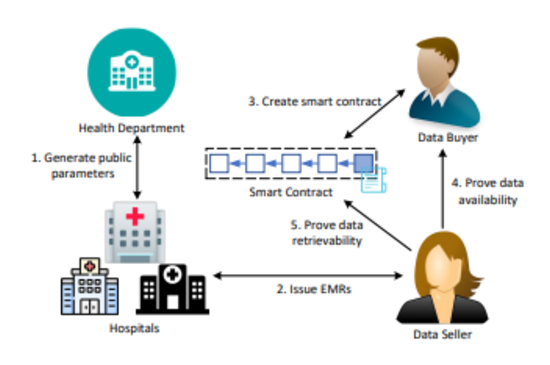
\includegraphics[width=0.96\linewidth]{imgs/23-network-model.eps}
  \caption{Network model~\cite{xue2023blockchain}}
  \label{fig:network_model}
  %\vspace{-5mm}
\end{figure}

\begin{figure}
\centering
  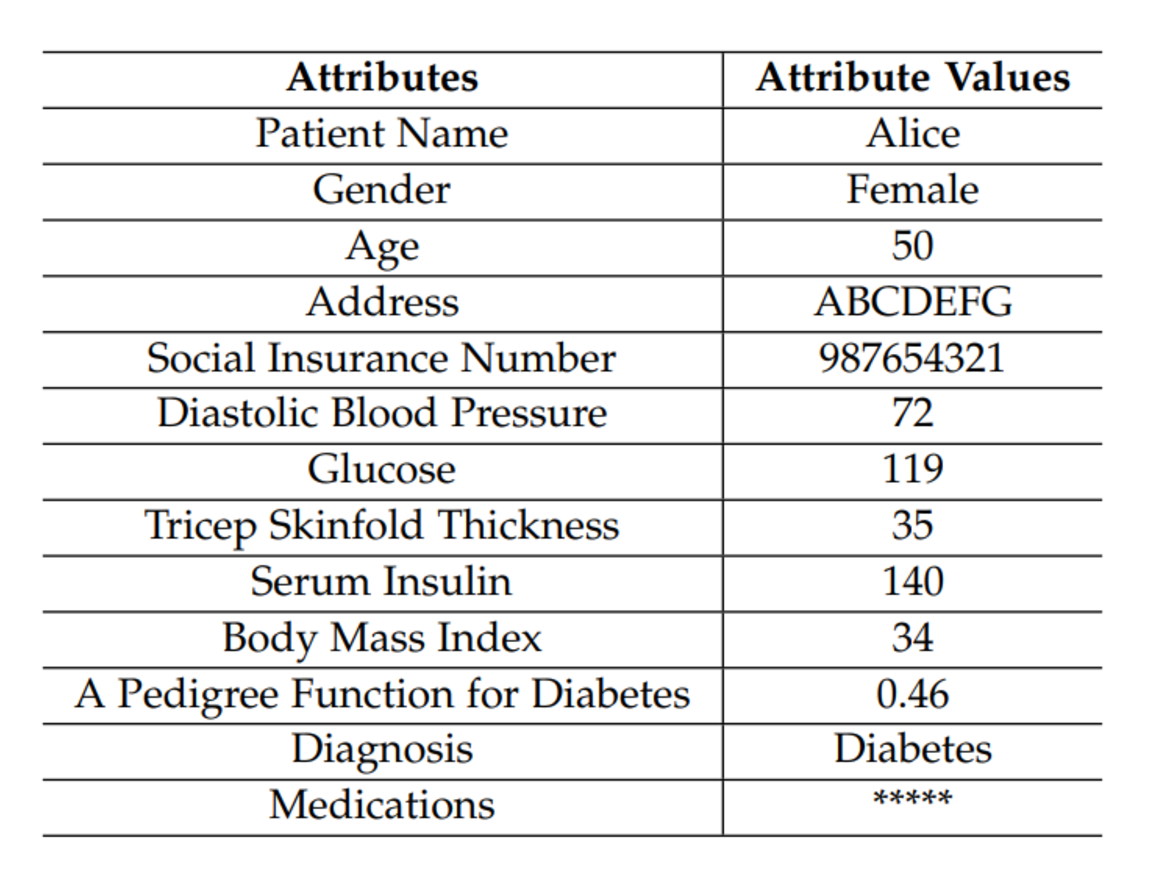
\includegraphics[width=0.8\linewidth]{imgs/23-example-emr-report.eps}
  \caption{An example EMR report~\cite{xue2023blockchain}}
  \label{fig:example-emr-report}
  %\vspace{-5mm}
\end{figure}

\subsubsection{Contributions}
The contributions of this paper are as follows:
\begin{itemize}
    \item Present a strategy for the data seller to sell the EMR report in parts (individual attributes), without affecting the ability of their verification
    \item Data fields attributes are signed by the hospital to ensure the integrity of the EMR reports while hiding the real identity of the hospital from the data buyer
\end{itemize}

\subsubsection{Threat Model}
In this paper, HD and hospitals are honest.
Data sellers and buyers can be malicious, as for data sellers, they want to gain as much money from data buyers as they could.
On the other hand, data buyers want to get access to the EMR reports without paying or get access to private information about the patients or the hospitals that they are not supposed to have access to.

\subsubsection{Used Schemes}
The paper uses the following building blocks:

\begin{itemize}
    \item \textbf{Structure-preserving Signature}~\cite{gay2018more}: A signature scheme that offers signature randomization and proved to be efficient in verification. That is why it is used in blockchain applications
    \item \textbf{ZKP}: This scheme is used to prove knowledge of correct encryption of the EMR report by the seller without revealing the encryption secret key to the buyer
    \item \textbf{Merkle Hash Tree}: This structure is used to hash the attributes inside an EMR report to prove that the attributes are related to the same report
    \item \textbf{AES}: This scheme is used to encrypt the attributes with a symmetric key $k$
    \item \textbf{El-gamal Encryption}: This scheme is used to encrypt the symmetric key $k$ using the buyer's public key
\end{itemize}

\subsubsection{Solution Overview}

In this section, the solution suggested in the paper is summarized, as shown in~\cref{fig:23-interactions-through-smart-contract} and following the example presented in \cref{sec:2023-problem-definition}:

\begin{itemize}
    \item \textbf{Policy Definition}: If the data buyer wants to gather EMR reports related to diabetes, then a smart contract will be initiated by him stating the requirements in terms of mandatory attribute values in the report and the attributes required to be gathered from the seller and signs them. 
    In this case, the attribute value \textit{Disease} shall have the value \textit{diabetes}, and the attribute required to be collected from the users are: \textit{Glucose, Diastolic Blood Pressure, Serum Insulin, and Age}. 
    In addition, he deposits the data reward to the smart contract
    \item \textbf{Policy Verification}: If the data seller has the required attributes, she verifies the signature on the required attributes using the buyer's public key
    \item \textbf{Present}: The data seller proves that she has the required data by sending the signature on the attributes, the ciphertext of the attribute values $CB$, and a ZKP of the correct encryption
    \item The smart contract checks the proof that the data seller has the required legitimate attributes, as posted by the data seller. 
    Then it sends a notification to the data buyer, who will recheck the proof and that the data seller meets the requirements posted in the definition of the policy, then he sends a confirmation message $CM$ to the smart contract
    \item \textbf{Ciphertext Generation}: The data seller encrypts the attributes encryption key $k$ with the buyer's public key $bpk$ to form the ciphertext $CK`$. 
    She sends the ciphertext with the ZKP of the correct encryption $\pi_b$ to the smart contract
    \item \textbf{Ciphertext Retrieval}: The smart contract checks the validity of the proof and sends a notification to the data buyer. 
    Afterward, The data buyer retrieves the ciphertext key and decrypts $CB$ to get the attribute values required
\end{itemize}

\begin{figure}
\centering
  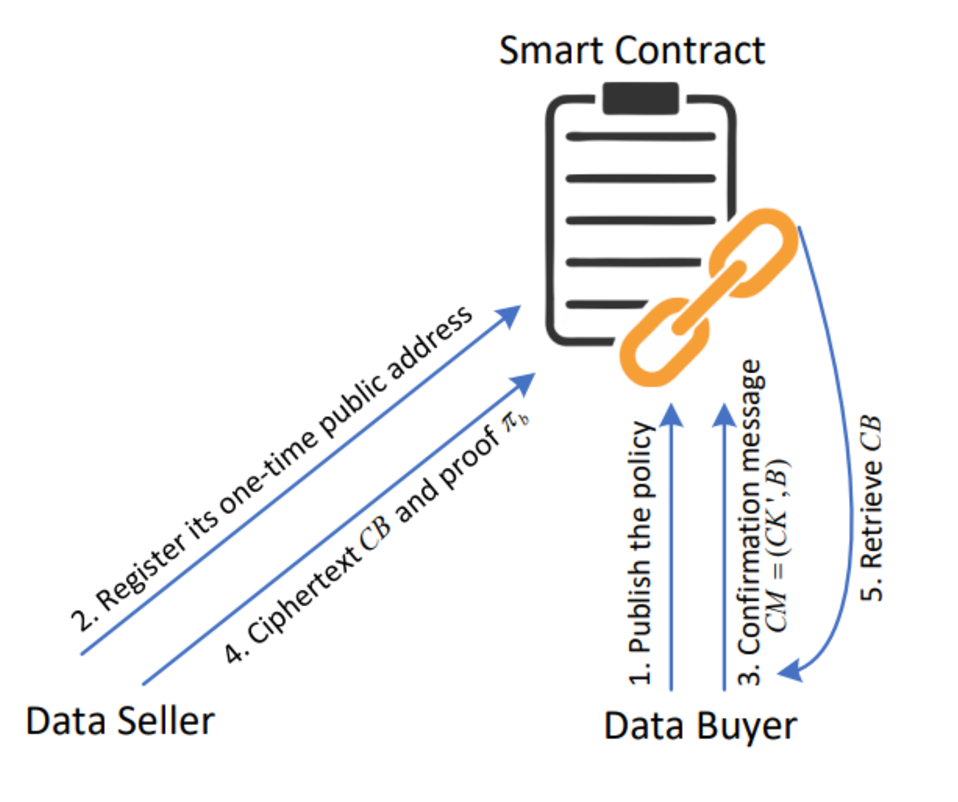
\includegraphics[width=0.8\linewidth]{imgs/23-interactions.eps}
  \caption{Interactions through the smart contract~\cite{xue2023blockchain}}
  \label{fig:23-interactions-through-smart-contract}
  %\vspace{-5mm}
\end{figure}

\subsection{Blockchain-cloud transparent data marketing: Consortium management and fairness~\cite{liu2022blockchain}}
\label{sec:blockchain-cloud-trasparent-data-marketing-consortium-management}

\subsubsection{Problem Definition and Network Model}
In IoT data Marketplace, data owners $DS$ have IoT devices, and third-party buyers $TP$ want to buy these data to find the users’ interests and analyze the data for their own future benefits.
All data marketing operations should be effectively managed while keeping data confidentiality and user identity privacy on top of the requirements since all the operations are performed on the cloud.
In addition, the data marketplace shall provide fairness for both $DS$ and $TP$.
In other words, $DS$ should be paid well for selling their data and $TP$ should pay only if he receives the correct data.
Moreover, depending on a centralized server lacks transparency and fairness since this entity may be hacked or worse, corrupt.
In the end, a fair and transparent data marketplace that depends on distributed management is a necessity.

The network model presented in this paper is shown in~\cref{fig:22-network-model}.
The consortium blockchain consists of a distributed set of supervising nodes to offer fairness and transparency.
Whereas the cloud server CS acts as an efficient data management unit where access to its data is controlled by the supervising nodes.
CS shall check the validity of the commitments of the data stored on its servers whenever new data is submitted to be stored by a DS. 
Those commitments prove the authenticity of the data stored on CS and that this data belongs to DS.

\begin{figure}
\centering
  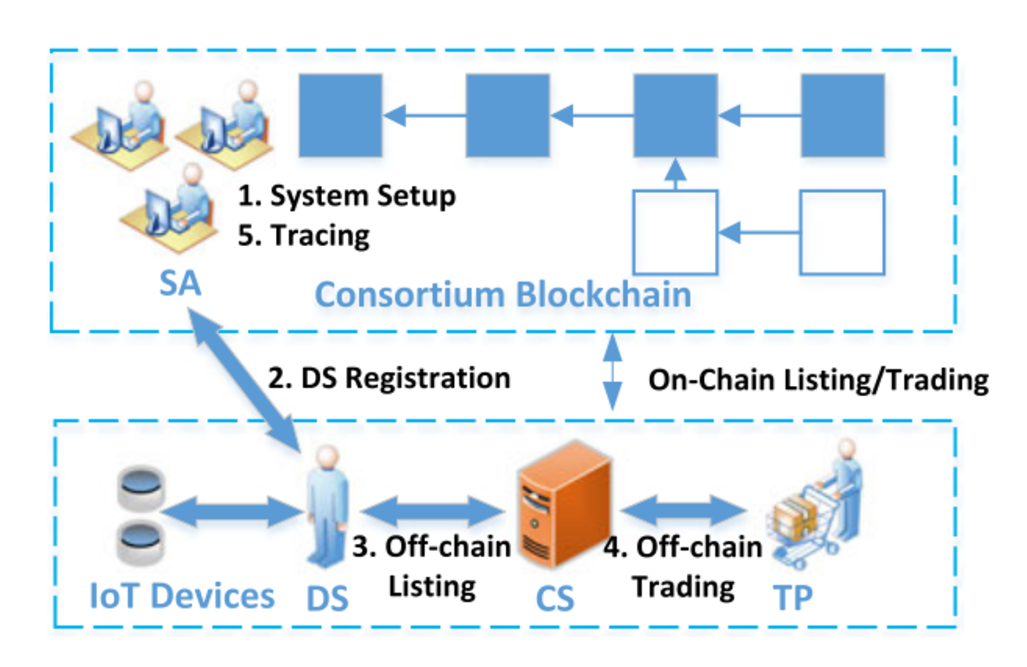
\includegraphics[width=0.9\linewidth]{imgs/22-network-model.eps}
  \caption{Network model~\cite{liu2022blockchain}}
  \label{fig:22-network-model}
  %\vspace{-5mm}
\end{figure}

\subsubsection{Contributions}

This paper presents a data marketplace exchange mechanism using blockchain technology and a cloud server which are managed by consortium management to ensure fairness and transparency.
The contributions of this paper can be summarized as follows:

\begin{itemize}
    \item A hybrid fair data marketing architecture is introduced that is based on a cloud server and a consortium blockchain.
    By financial incentives and succinct ‘commitments’ of marketing operations, the protocol can achieve marketing fairness and effective detection of unfair marketing operations
    \item The requirements of GDPR are all met
    \item The identity of the data owners $DS$ is preserved with the ability to expose any malicious users by the consortium management 
\end{itemize}

\subsubsection{Threat Model}

In this paper, CS may be malicious that he won't check the validity of the commitments submitted by DS because its goal is to maximize its profit regardless of the correctness of the submitted data.
In addition, the blockchain is an immutable distributed storage that provides automatic contract executions.
TP is a rational party who wants to pay for the data he requests if the correctness of it is guaranteed.
Additionally, DS is also a rational user who wants to trade if the marketing requirements and fair payments are achieved.
Finally, SA consists of a set of trusted supervising nodes.

\subsubsection{Used Schemes}
The paper depends on the following primitives in its solution:

\begin{itemize}
    \item \textbf{ZKP}: This scheme is used for the seller to prove knowledge of a secret without revealing the secret itself to the buyer
    \item \textbf{PVSS}~\cite{schoenmakers1999simple}: A $(t,n)$ PVSS scheme enables a dealer holding a secret s to share the secret with n participants $(P_1, P_2, ..., P_n)$, where t-out-of-n participants can later combine the shares and recover the secret. In this paper, the seller splits his secret identity into $n$ secret shares that he shares with the supervising nodes. Later, if the user shows a malicious activity, $t$ out of $n$ supervising nodes can collaborate to reveal his real identity using those secret shares
    \item \textbf{PS Signature}~\cite{pointcheval2018reassessing}: A short signature scheme with a randomized verification mechanism. In this paper, after the secret shares are sent by the seller to the supervising nodes as discussed in the PVSS scheme, each supervising node signs his own share and returns it back to the seller. After that, the seller aggregates the signatures he gets from the supervising nodes on the secret shares. The output of the signature aggregation process is the user's anonymous identity
    \item \textbf{El-gamal Encryption}: This scheme is used to encrypt the symmetric key used by the seller to encrypt his plain data
    \item \textbf{AES}
\end{itemize}

\subsubsection{Solution Overview}
The solution provided in the paper can be summarized in five main steps, as follows:

\begin{itemize}
    \item \textbf{System Setup}: SA initializes a consortium blockchain network and sets the public parameters. 
    In addition, the public and private keys for each SA are set up for the schemes: PS, PVSS, and Elgamal
    \item \textbf{Registration}: TP and CS register themselves to get a membership to access the blockchain.
    Moreover, DS registers himself as shown in~\cref{fig:22-ds-registration}
    \item \textbf{Off-chain Data Listing}: The sequence diagram for DS to list the data item that she wants to trade inside CS is shown in~\cref{fig:22-off-chain-data-listing}
    \item \textbf{On/Off-chain Trading}: The sequence diagram for DS to trade with TP using the smart contract is depicted in~\cref{fig:22-off-chain-trading}
    \item \textbf{User Tracing}: The identity of DS should be traced and exposed in the following cases.
    First, If the commitments submitted by DS are not valid when checked against the data items listed in the CS.
    Second, If TP finds that the description of the file after decryption does not match the description originally submitted by DS when the smart contract was created.
    If any of these conditions apply, the supervising nodes cooperate together to reveal the identity of DS following $PVSS.Recover$ algorithm
\end{itemize}

\begin{figure}
\centering
  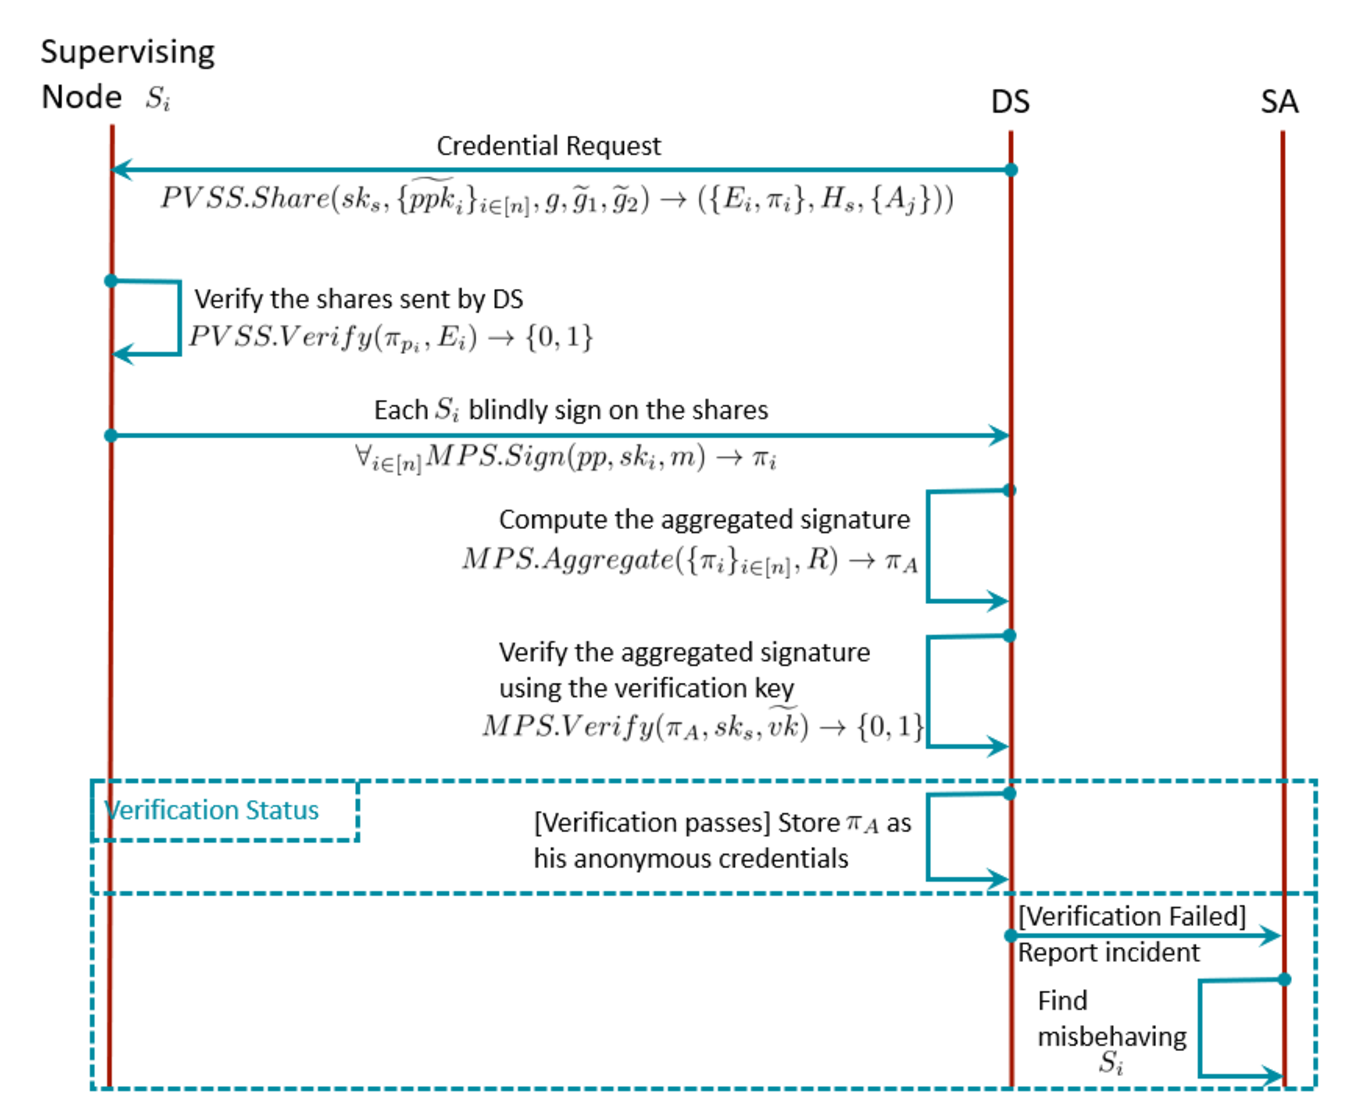
\includegraphics[width=1\linewidth]{imgs/22-sequenceRegisterDs.eps}
  \caption{DS registration}
  \label{fig:22-ds-registration}
  %\vspace{-5mm}
\end{figure}

\begin{figure}
\centering
  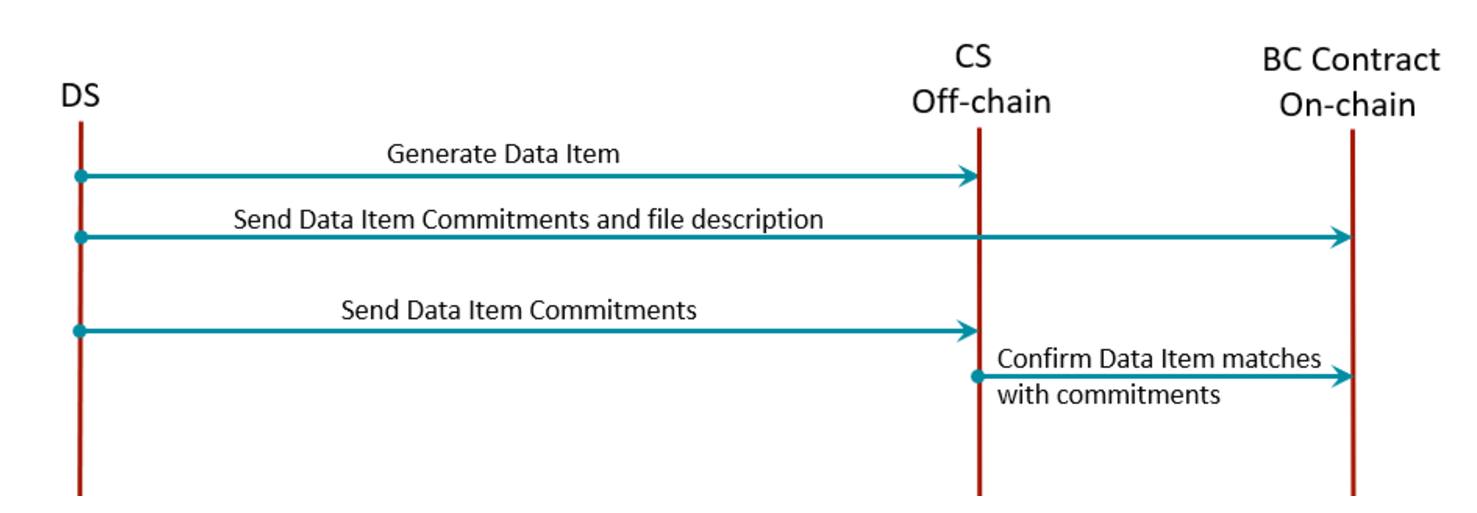
\includegraphics[width=1\linewidth]{imgs/22-sequenceDataListing.eps}
  \caption{Off-chain data listing}
  \label{fig:22-off-chain-data-listing}
  %\vspace{-5mm}
\end{figure}

\begin{figure*}
\centering
  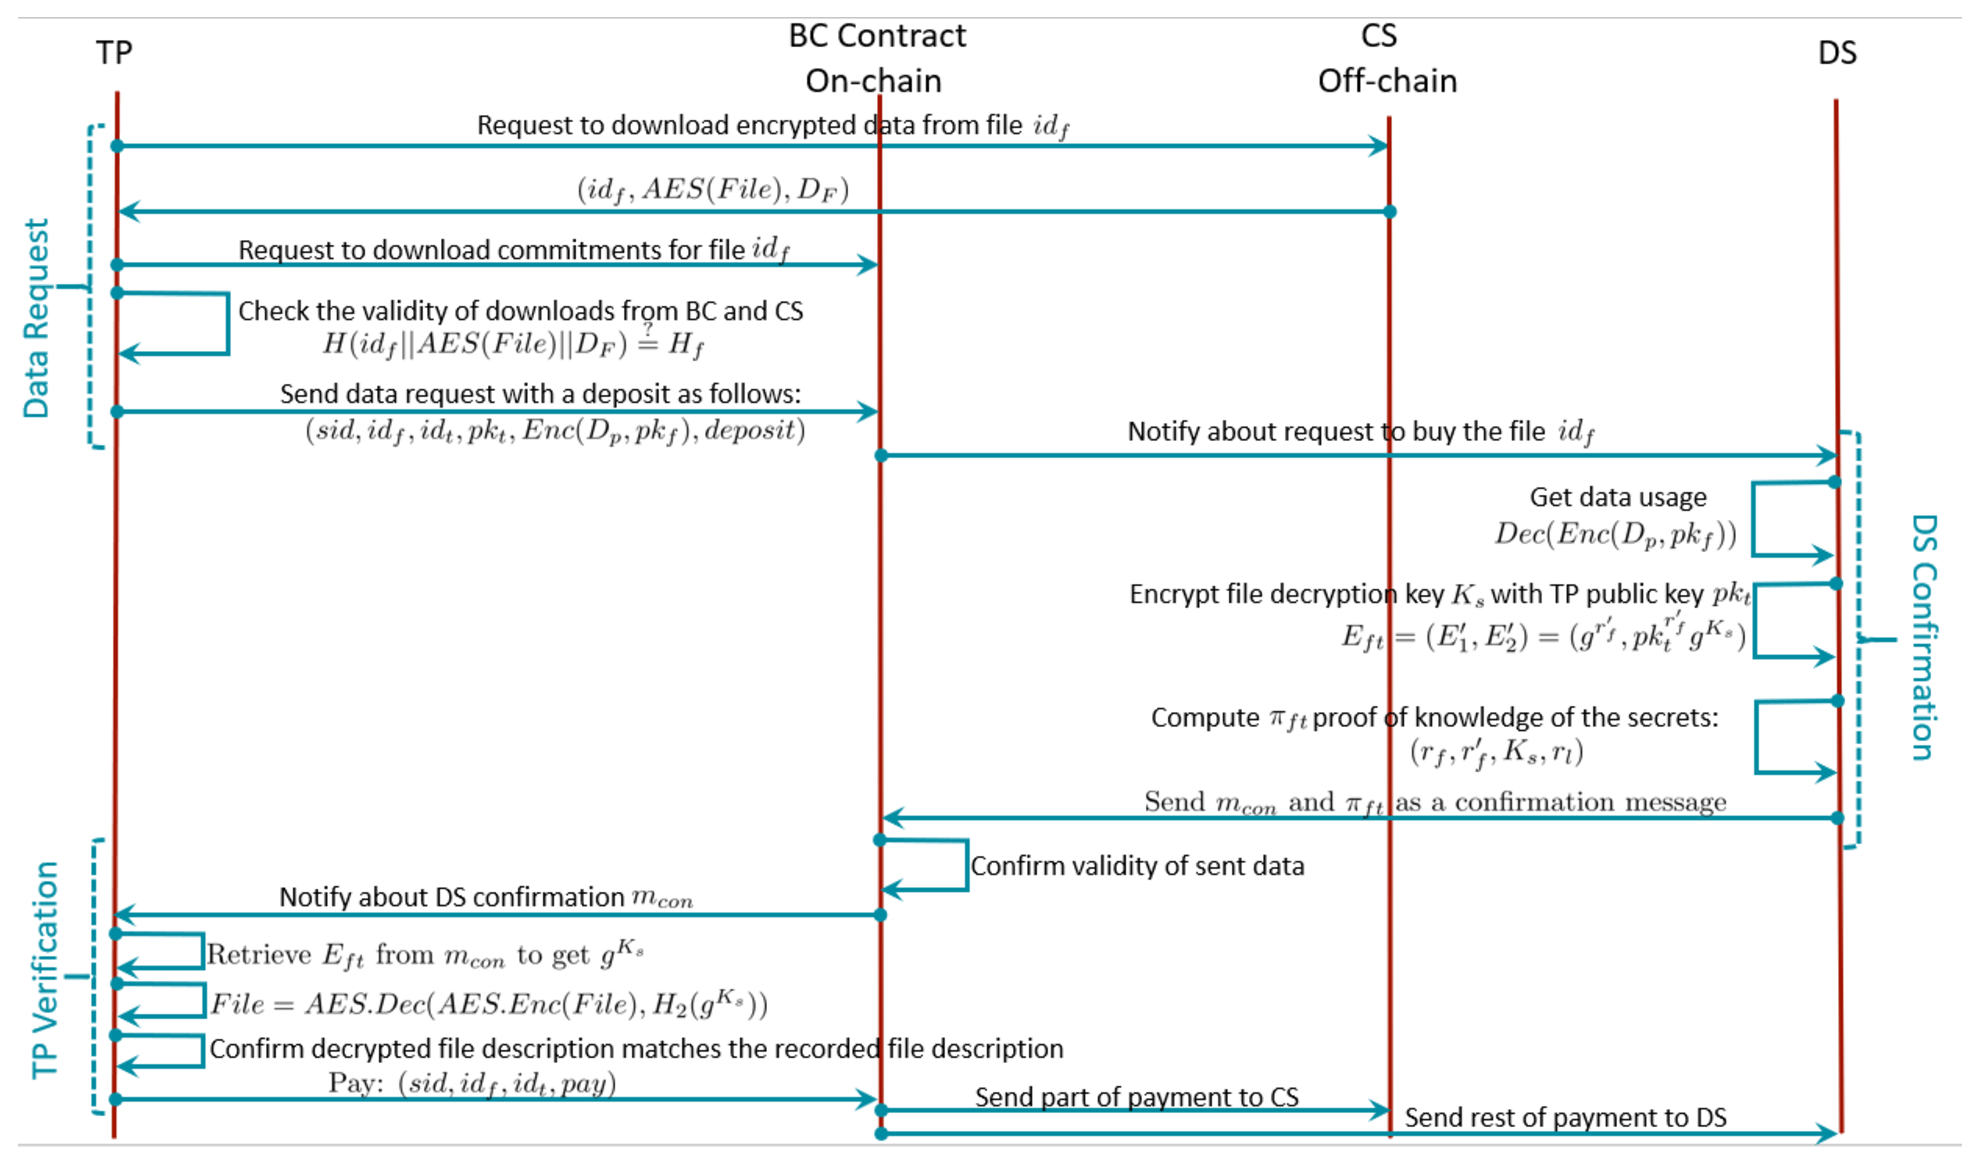
\includegraphics[width=1\linewidth]{imgs/22-sequenceTrading.eps}
  \caption{On/Off-chain trading}
  \label{fig:22-off-chain-trading}
  %\vspace{-5mm}
\end{figure*}

\subsection{A Blockchain-based Medical Data Marketplace with Trustless Fair Exchange and Access~\cite{alsharif2020blockchain}}
\label{sec:blockchain-based-medical-data-marketplace-20}

\subsubsection{Problem Definition and Network Model}
High demand for clinical research necessitates novel medical data marketplaces to facilitate medical data and records trading between medical data sellers and interested buyers in a secure manner.
Therefore, flexible access control should be considered when designing such a marketplace.
For example, some sellers may be interested to sell their medical records to research institutes only within some predefined geographical areas.

\Cref{fig:20-network-model} shows the network model presented in the paper.
KDC initializes the global parameters and provides all entities with their public/private key pairs.
In addition, it provided the buyers with their attributes and the corresponding decryption key for each attribute.
The blockchain network stores and executes smart contracts initiated by sellers.
Moreover, the peer-to-peer network is used to store off-chain encrypted data by sellers.


\subsubsection{Contributions}
In this paper, the authors propose a model for medical data marketplace with flexible access control that is based on a trustless environment.
In particular, they developed a mechanism to enable sellers to enforce an access control policy on the encrypted records using CP-ABE while allowing buyers to verify the correctness of the encrypted records using ZK-SNARK protocol.

\begin{figure}
\centering
  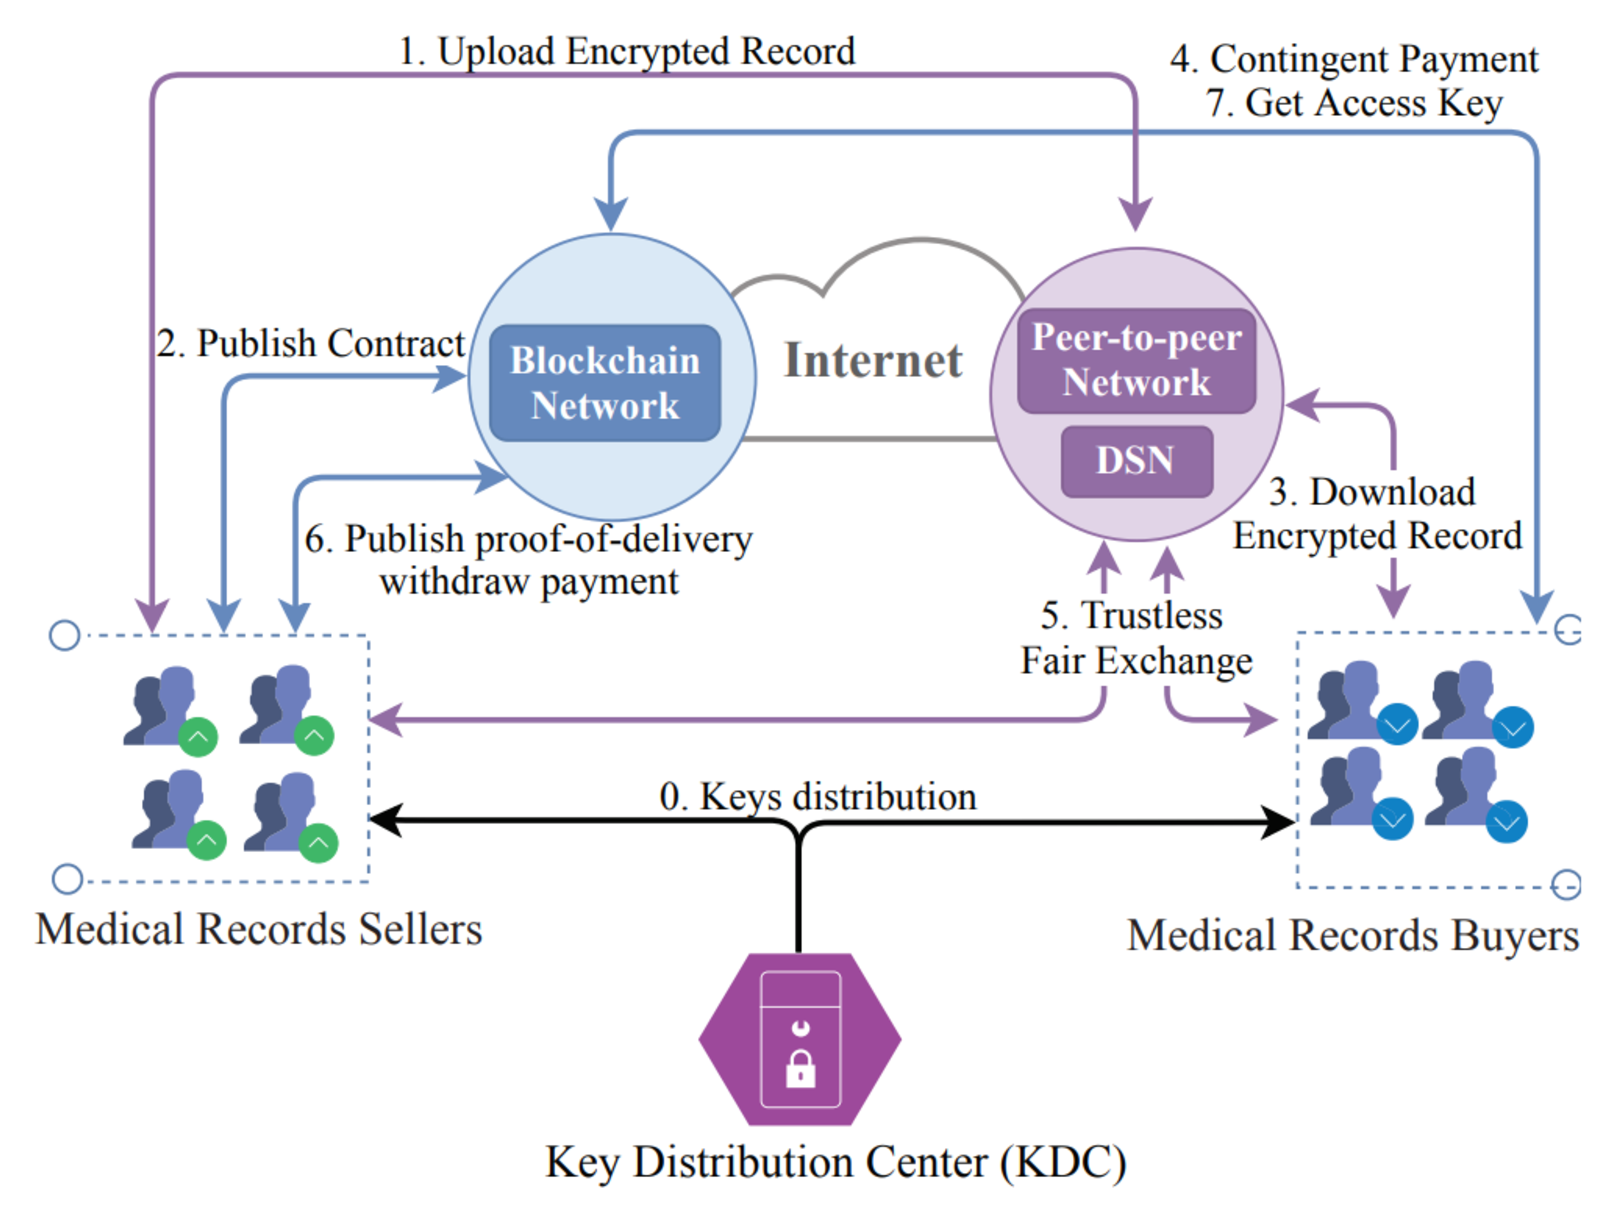
\includegraphics[width=1\linewidth]{imgs/20-network-model.eps}
  \caption{Network model~\cite{alsharif2020blockchain}}
  \label{fig:20-network-model}
  %\vspace{-5mm}
\end{figure}

\subsubsection{Threat Model}
Both sellers and buyers can be malicious users.
Towards this direction, a seller may try to claim a payment from a buyer without providing the correct access key to the encrypted medical records.
Comparatively, a buyer may also want to have access to the medical records without paying the seller its due amount.
Finally, the medical records are assumed to be authentic and they cannot be forged.

\subsubsection{Used Schemes}
In this paper, the following security primitives were used:

\begin{itemize}
    \item \textbf{CP-ABE}~\cite{bethencourt2007ciphertext}: Each entity is given a set of attributes that defines its identity.
    Afterwards, anyone can generate a ciphertext that is associated with an access policy defined over those attributes.
    Only the users who satisfy the access policy can decrypt the message
    \item \textbf{ZK-SNARKs}~\cite{ben2013succinct}: It is an efficient and secure non-interactive protocol that allows a verifier to attest the untrusted prover knowledge of some secret inputs, called witnesses without revealing the secret inputs to anyone
    \item \textbf{AES}
\end{itemize}

\subsubsection{Solution Overview}
The solution provided in this paper comprises five steps.

\begin{itemize}
    \item \textbf{System Setup}: KDC generates the public/private key pairs for all users and assigns the attributes and the associated decryption keys to each buyer according to his identity
    \item \textbf{Medical Records Encryption and Upload}:  The seller encrypts a record with the AES scheme, uploads it to the DSN network, then registers itself as the owner of this data item
    \item \textbf{Document's Access Policy Creation}: The seller defines the access policy as a boolean expression over the set of attributes.
    In addition, it creates proof of knowledge $\pi^{PoE}$ that proves correct encryption under the AES scheme and proves knowledge of the secret shares used to construct the access policy.
    In the end, the seller initiates the smart contract with the address of the encrypted data on the peer-to-peer network and the file commitments
    \item \textbf{Contingent Payment Deposit by Buyer}: The buyer browses the listings on the peer-to-peer network, downloads the encrypted file and the commitments for the file that he wants to buy, and verifies the correctness using the ZKP verification scheme.
    Finally, the buyer deposits a contingent payment to the smart contract
    \item \textbf{Off-chain Trustless Fair Exchange}: First, the buyer contacts the seller using the peer-to-peer network and sends him his public key.
    Second, the seller verifies that the buyer's public key is listed in the pending requests on the smart contract, then she sends her public key to the buyer with a challenge for him to sign.
    Third, after the buyer signs the challenge and sends it back to the seller, the seller verifies the correctness of the signature
    Forth, the seller sends the hash of the secret value $hg$ as long as a proof of delivery $\pi^{PoD}$.
    Fifth, the buyer verifies the correctness of the $\pi^{PoD}$ and signs on the the hash value $hg$
    \item \textbf{Payment Withdraw}: The seller verifies the signature of the buyer, then he can send a redemption transaction request to the smart contract
    \item \textbf{Access Control and Document Decryption}: After payment withdrawal, the buyer can read the secret value whose hash is $hg$ from the smart contract, which was the last piece in the puzzle needed to recover AES decryption key used to encrypt the document following CP-ABE decryption algorithm
    
\end{itemize}

\section{Schemes Comparison}
\label{sec:schemes-comparison}

In this section, we compare the three presented papers.
It is also worth mentioning that all three papers use smart contract-based blockchain networks.
In~\cref{tab:general-comparison}, we present a general comparison between 
the three papers in terms of GDPR requirements compliance, domain, and blockchain characteristics.
Moreover, \cref{tab:used-primitives-comparison} shows the primitives used in each paper.

\begin{table*}[h!]\centering
\caption{General schemes comparison}\label{tab:general-comparison}
\scriptsize
\begin{threeparttable}
\begin{tabular}{lrrrrrrrr}\toprule
&R2I\tnote{1} &R2C\tnote{2} &Hide Seller's Identity &Fine Grained Data &Domain &Blockchain Type &On/Off-chain Model \\\midrule
\cite{xue2023blockchain} &Yes &Yes &Yes &Yes &Medical &Not mentioned\tnote{4} &On-chain \\
\cite{liu2022blockchain} &Yes &Yes &Yes (conditional)\tnote{3} &No &\ac{iot} &Consortium &On/Off-chain \\
\cite{alsharif2020blockchain} &Yes &Yes &No &No &Medical &Public &On/Off-chain \\
\bottomrule
\end{tabular}
\begin{tablenotes}
    \item[1] R2I: Right of the Seller to be informed
    \item[2] R2C: Right of the seller to control her listed data
    \item[3] Conditional means: with the ability to expose the misbehaving seller
    \item[4] We see that the blockchain can be public or private
\end{tablenotes}
\end{threeparttable}
\end{table*}

\begin{table*}[h!]\centering
\caption{Used primitives comparison}\label{tab:used-primitives-comparison}
\scriptsize
\begin{threeparttable}
\begin{tabular}{lrrrrrrrr}
\toprule % Add a line on top of the table
&\ac{zkp} &Signature &PVSS &Symmetric Encryption &Asymmetric Encryption &CP-ABE &Merkle Hash Tree \\\midrule
\cite{xue2023blockchain} &Fiat-Shamir &Structure preserving signature &No &\ac{aes} &Elgamal &No &Yes \\
\cite{liu2022blockchain} &Fiat-Shamir &PS Signature &Yes &\ac{aes} &Elgamal &No &No \\
\cite{alsharif2020blockchain} &ZK-SNARK &Yes\tnote{1} &No &\ac{aes} &No &Yes &No \\
\bottomrule
\end{tabular}
\begin{tablenotes}
    \item[1] No specific signature scheme was mentioned
\end{tablenotes}
\end{threeparttable}
\end{table*}



\section{Conclusions and Future Work}
\label{sec:conclusions}
% Conclusion
In this paper, security, privacy, and fairness issues in the blockchain-based marketplace in two major domains were studied.
In addition, a comprehensive review of privacy preservation and incentive fairness were provided.
Furthermore, several approaches to deal with security, privacy, and fairness challenges were described.
% Future directions
Finally, the future direction in this field can be concluded as follows.
First, anonymity shall be provided to all involved parties while having the possibility of revealing the real identity of a misbehaving party by consortium management.
Second, different \ac{zkp} techniques emerge to prove knowledge of the secrets without revealing them to the verifying parties.
Third, trading parts of verifiable records without exposing the whole data in the original records is a must.


\bibliographystyle{IEEEtran}
\bibliography{tex/review.bib}

\end{document} 